\documentclass{rapport}
\usepackage{lipsum}
\usepackage{gensymb}
\usepackage{float}
\usepackage{graphicx} % Required for inserting images
\usepackage{pythontex}
\usepackage{setspace}
\usepackage[skip=0pt]{caption}
\usepackage{booktabs}
\usepackage{tabularx}
\usepackage{amsmath}


\title{file title} %title of the file

\begin{document}
\onehalfspacing

%----------- Report information ---------

\logo{logos/DTU_Logo_Roed.jpg}
\uni{\textbf{Technical University of Denmark}}
\ttitle{BMI 2} %title of the file
\subject{Subject} % Subject name
\topic{Assignment 2} % Topic name

\students{\textsc{Visnukaran Kirubakaran, Student ID: s224527}} % information related to the students

%----------- Init -------------------
        
\buildmargins % display margins
\buildcover % create the front cover of the document
\toc % creates the table of contents

%------------ Report body ----------------
\section{Statistical analysis}
\addcontentsline{toc}{subsubsection}{\textbf{a)} Description of the data material}
\subsubsection*{\textbf{a)} Description of the data material}
\noindent
In this project, data from the BMI study is analyzed, which aims to establish an appropriate multiple linear regression model for BMI. The provided dataset contains 847 observations, focusing on the following variables:

\begin{itemize}
    \item ID: The respondent's number (can be used for identification).
    \item BMI: The respondent's BMI (in kg/m²).
    \item Age: The respondent's age (in years).
    \item Fastfood: Frequency of the respondent's visits to fast-food restaurants (days/year).
\end{itemize}

\noindent
Additionally, a variable such as log(BMI), which is the logarithm of the BMI, is also added. This variable simplifies later calculations.
\noindent
This is a complete sample, as all values that are given are included. All the mentioned variables are quantitative, as the data is numerical, and can both be quantified and measured. Of the aforementioned variables, three are selected: log(BMI), age, and fastfood.
\noindent
For these three variables, we can create scatter plots where log(BMI) is plotted against age and fastfood to investigate the correlation between them.

\hspace{20 mm}

\noindent
On the following scatter plot of log(BMI) over age, it appears that there is no real correlation between the two factors. This can be observed from the scattered data.

\begin{figure}[H]
    \centering
    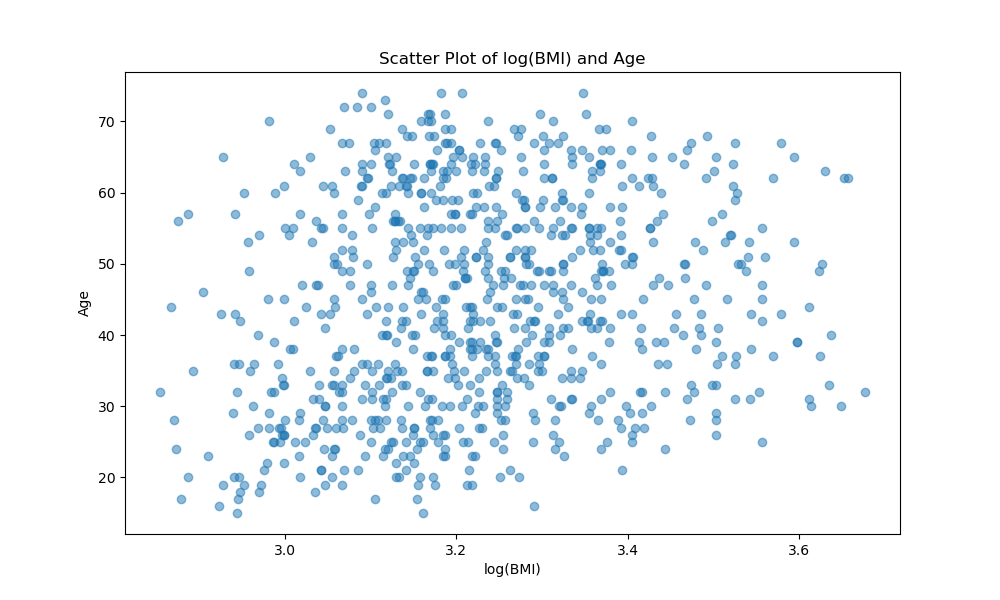
\includegraphics[width=0.75\textwidth]{Figures/scatter_plot_1.png}  % Set width to 75% of text width
    \caption{\small Scatterplot of log(BMI) and Age.}  % Use smaller font for the caption
    \label{fig:scatterplot_1}
\end{figure}
\noindent
\noindent
The same thing can be seen on the scatterplot of the log(BMI) and fastfood where it does not seem there is a correlation between BMI and fastfood, since the data is scattered. 

\begin{figure}[H]
    \centering
    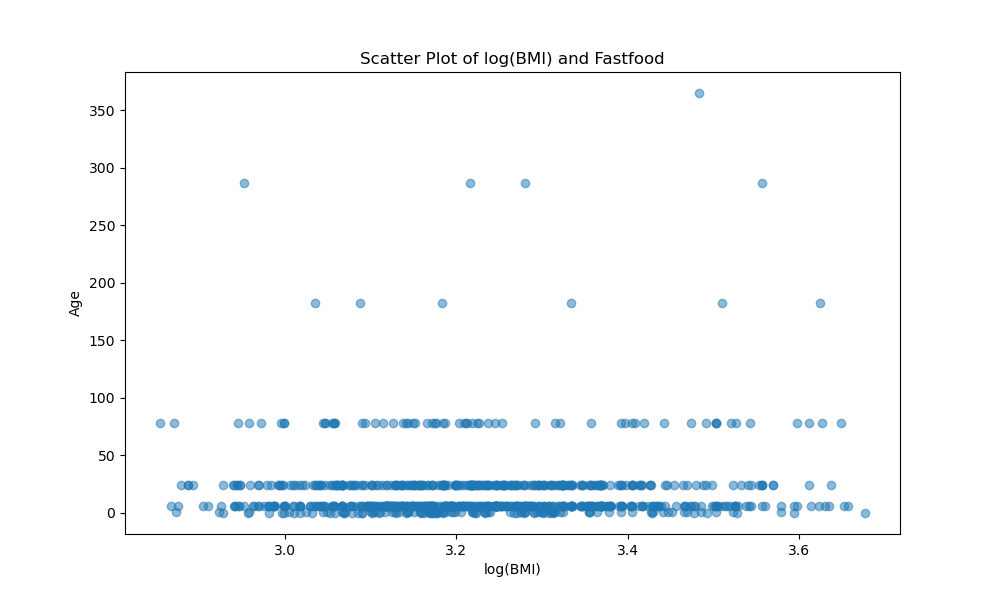
\includegraphics[width=0.75\textwidth]{Figures/scatter_plot_2.png}  % Set width to 75% of text width
    \caption{\small Scatterplot of log(BMI) and Fastfood.}  % Use smaller font for the caption
    \label{fig:scatterplot_1}
\end{figure}
\noindent
\noindent
Further, we undertake a graphical examination of each variable using histograms and box plots. 

\begin{figure}[H]
    \centering
    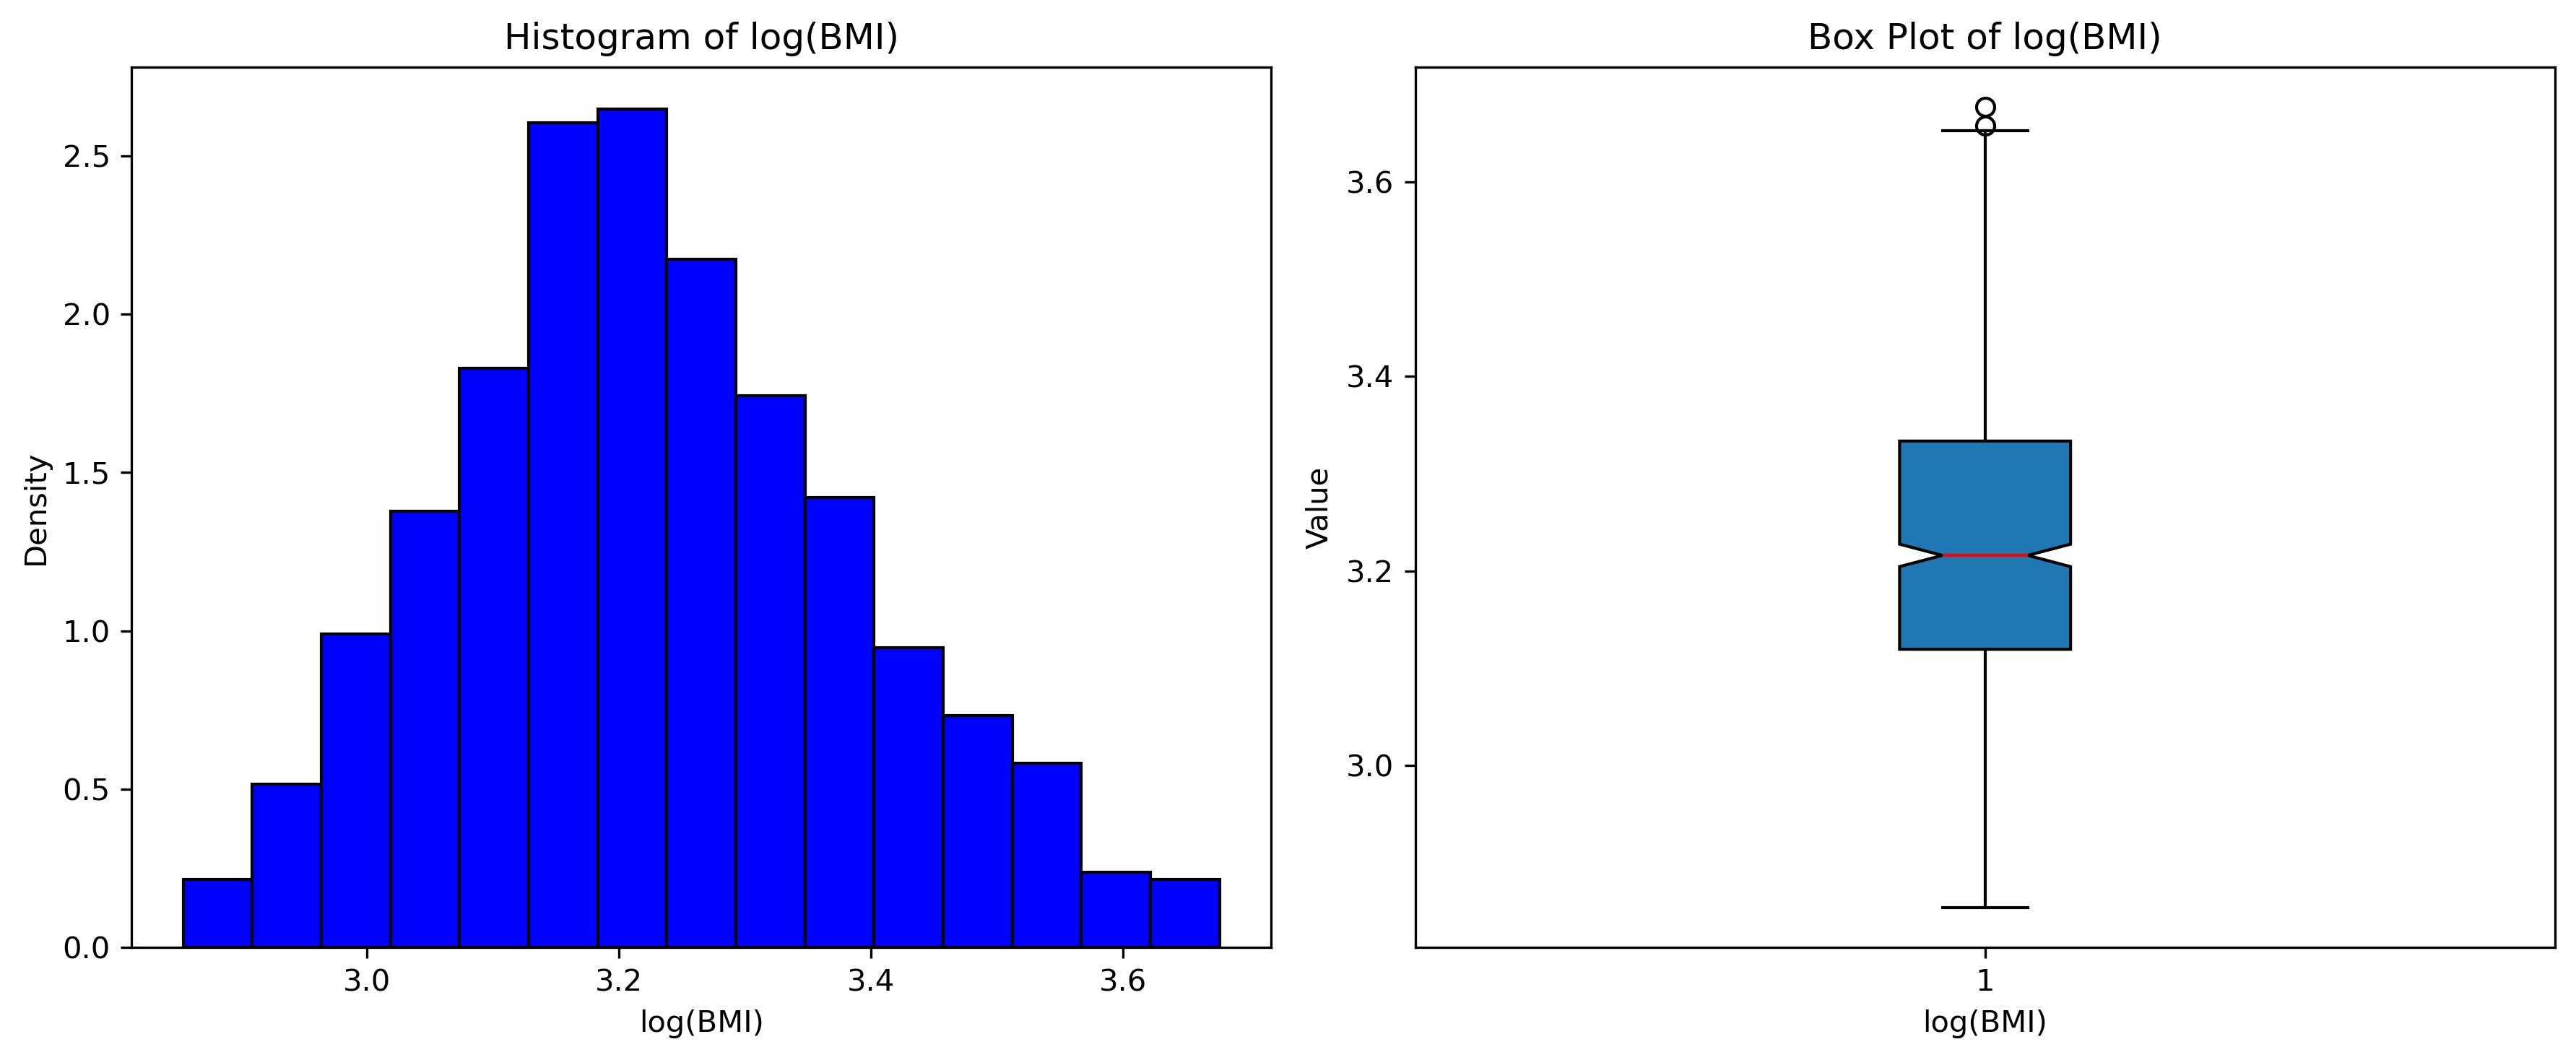
\includegraphics[width=0.75\textwidth]{logbmi_hist_box.png}
    \caption{\small Histogram and boxplot of log(BMI).}
    \label{fig:logbmi}
\end{figure}
\noindent
The histogram for log(BMI) indicates a tendency towards a normal distribution with some skewness. The boxplot highlights a median slightly above 3.2, suggesting a slight skew towards lower values. Notably, a couple of outliers are present on the upper end, indicating some deviations from a typical normal distribution.


\begin{figure}[H]
    \centering
    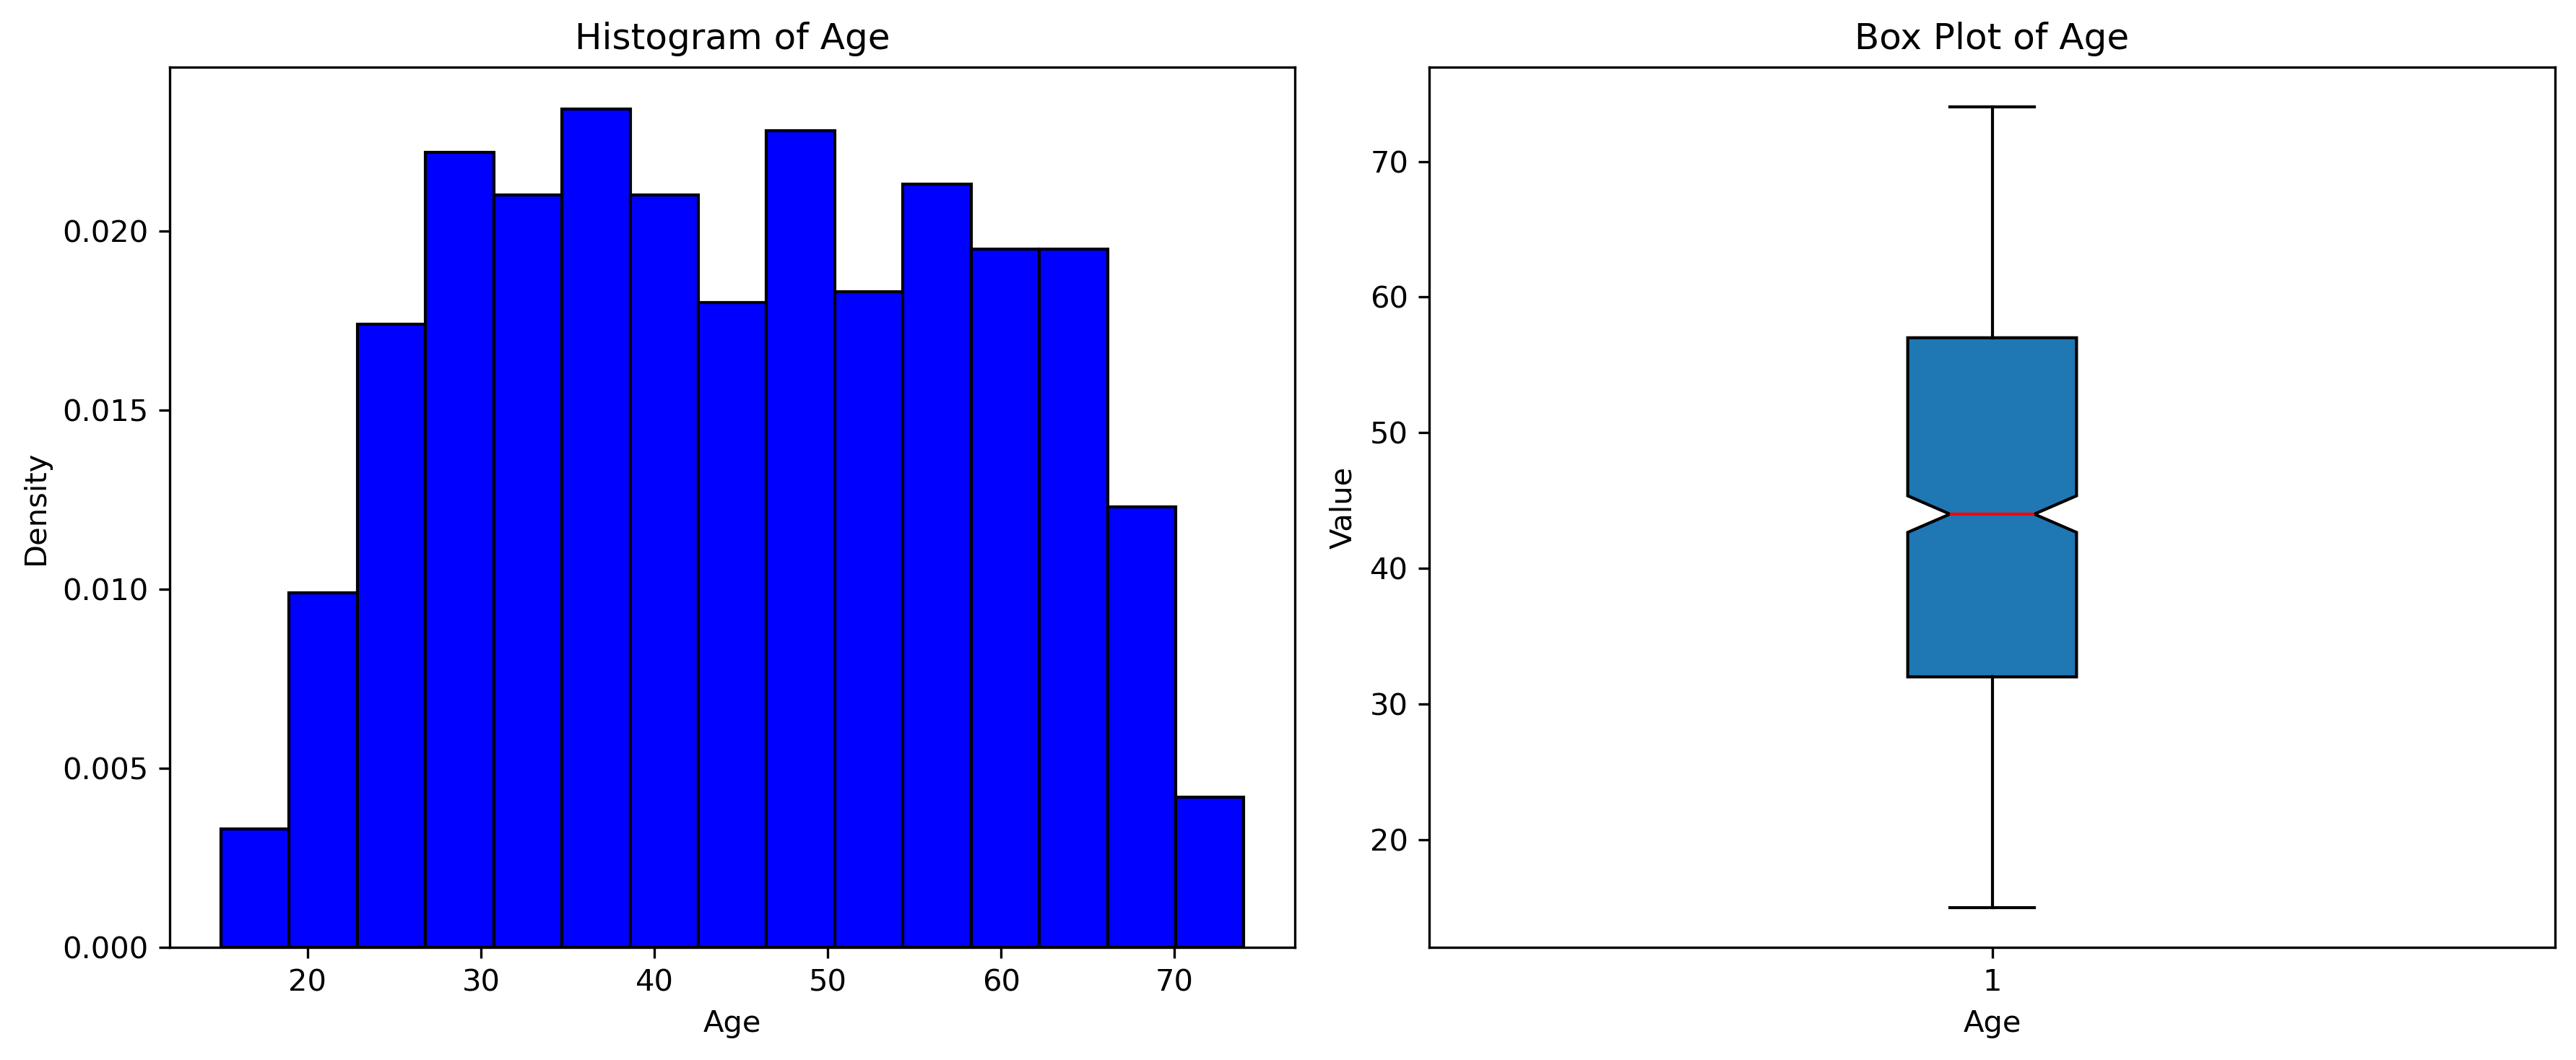
\includegraphics[width=0.75\textwidth]{age_hist_box.png}
    \caption{\small Histogram and boxplot of Age.}
    \label{fig:age}
\end{figure}
\noindent
The histogram for age reveals a broad spread of values, indicative of high variability within the age data. The boxplot shows a median value around 45, nicely centered between the quartiles, reflecting a balanced distribution despite the wide range. The plot suggests a fairly symmetric distribution of age, although the range suggests varied participant ages.


\begin{figure}[H]
    \centering
    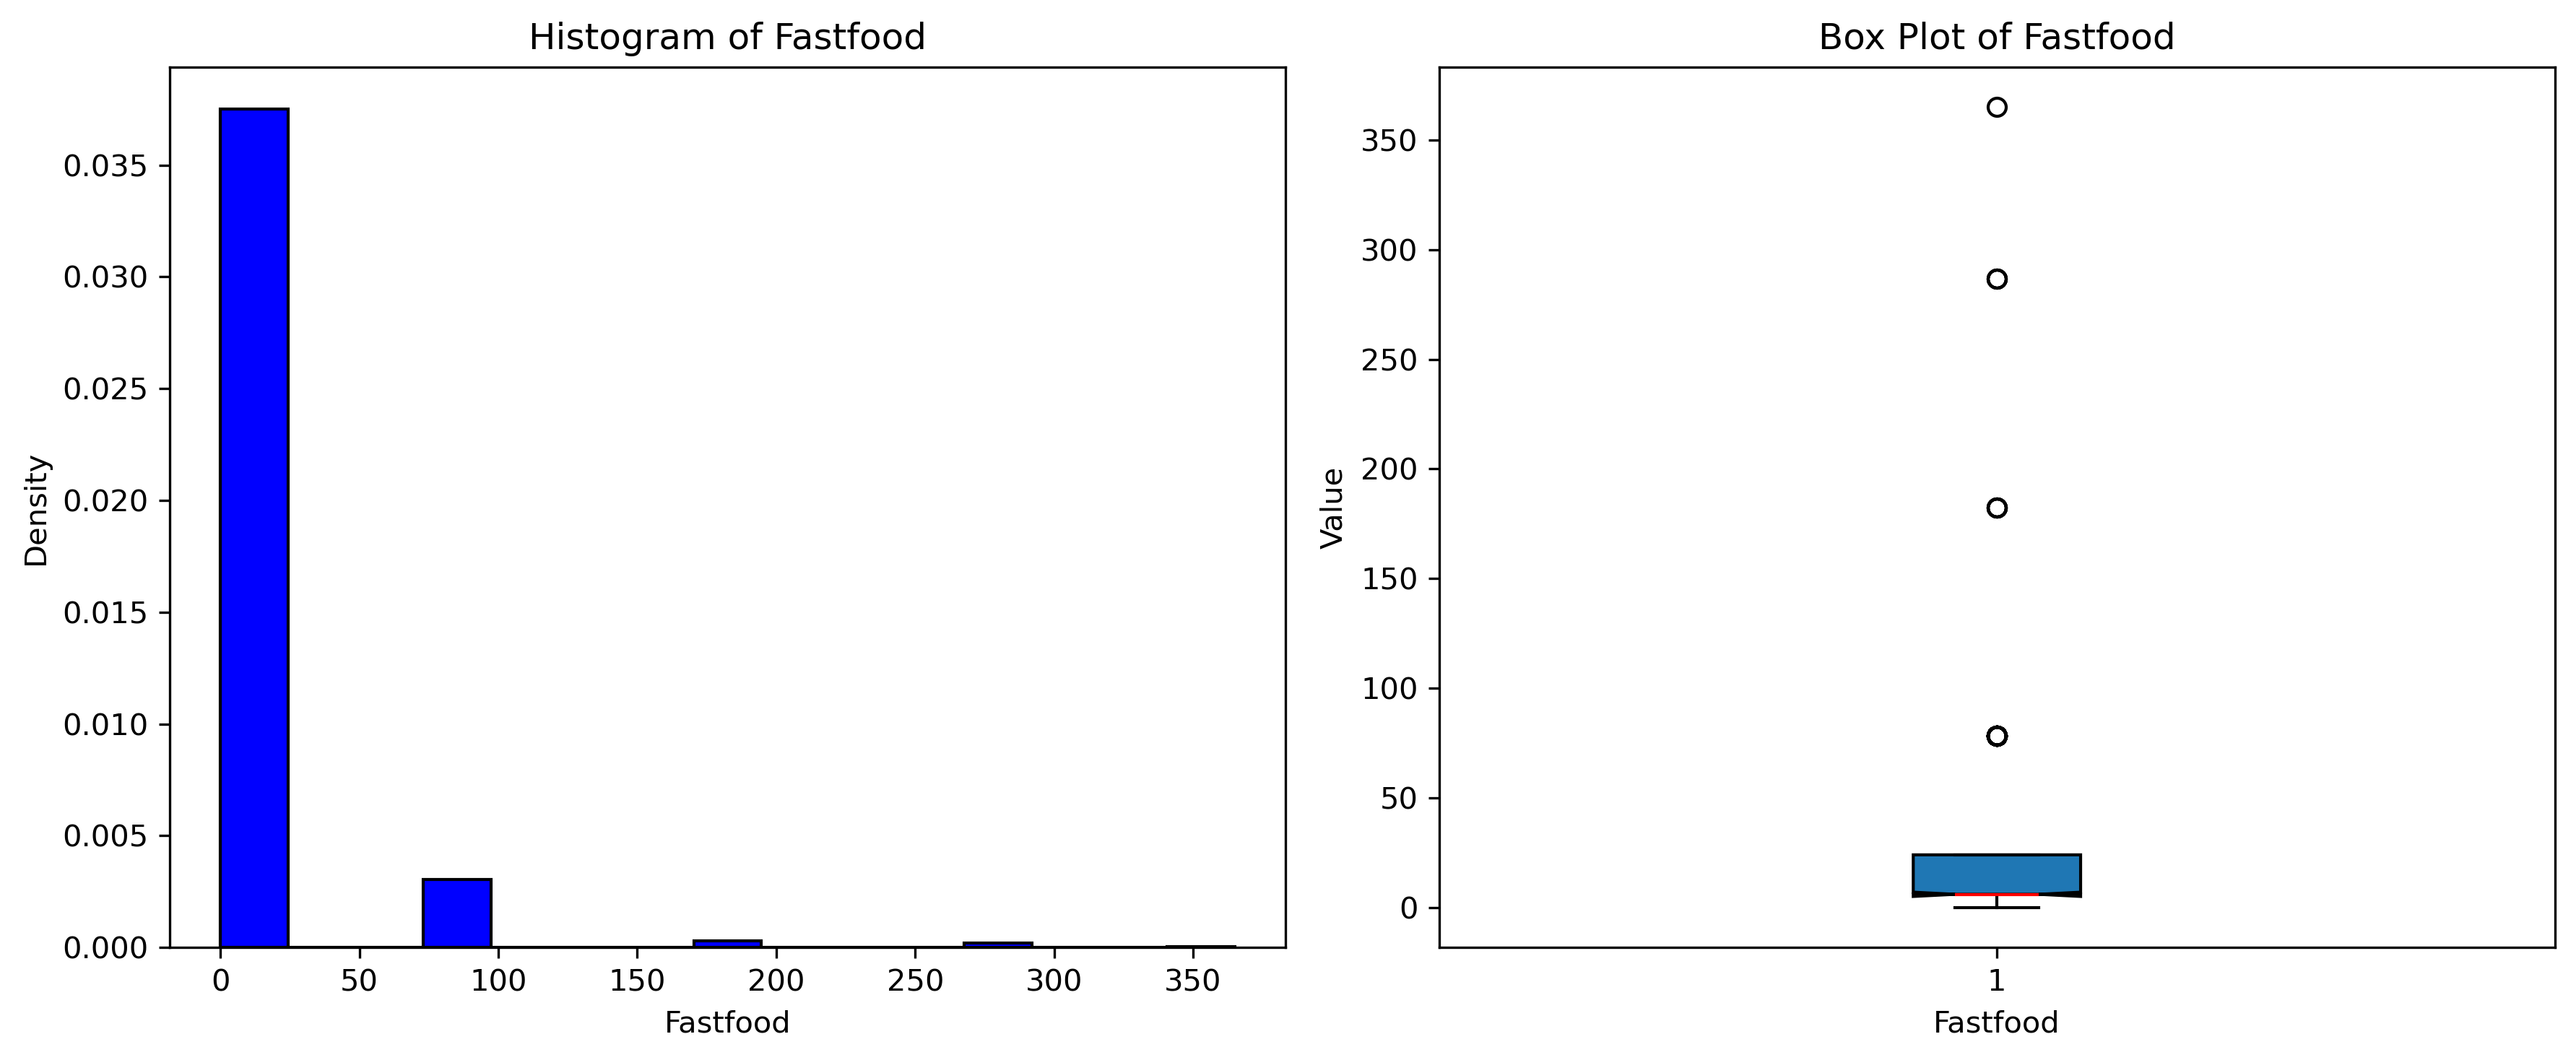
\includegraphics[width=0.75\textwidth]{fastfood_hist_box.png}
    \caption{\small Histogram and boxplot of Fastfood.}
    \label{fig:fastfood}
\end{figure}
\noindent
The fastfood consumption histogram clearly shows a concentration of data points below 100 days, with rare occurrences extending beyond this range. The corresponding boxplot underscores this concentration, with the bulk of data points situated at lower consumption levels. The median, close to the lower quartile, and several high-range outliers highlight the uneven distribution across the dataset.

All relevant data can be seen here:
\begin{figure}[H]
    \centering
    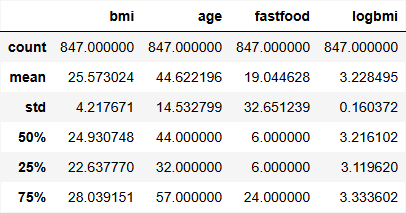
\includegraphics[width=0.8\textwidth]{summary_statistics.png}
    \caption{\small Summary statistics for the dataset.}
    \label{fig:summary_statistics}
\end{figure}

\noindent
The table in Figure displays the summary statistics of our main variables. These statistics provide essential insights into the distribution characteristics of each variable, including their central tendencies and variabilities. The median values, along with the first and third quartiles, are particularly helpful in understanding the asymmetry and potential outliers in the data. This detailed statistical overview aids in ensuring the robustness and reliability of subsequent analyses.





\addcontentsline{toc}{subsubsection}{\textbf{b)} Multiple linear regression model}
\subsubsection*{\textbf{b)} Multiple linear regression model}
\noindent
Now, we can formulate a multiple linear regression model with the log-transformed BMI scores
\noindent
as the dependent/outcome variable ($Y_i$), and age and fast-food consumption as
\noindent
the independent/explanatory variables ($x_{1,i}$, and $x_{2,i}$ respectively). 

$$
Y_i = \beta_0 + \beta_1x_{i1} + \dots + \beta_px_{ip} + \varepsilon_i, \quad \varepsilon_i \sim N(0, \sigma^2)
$$

\noindent
Here, we make the assumption that the residuals, $\varepsilon_i$, are all independent and identically distributed with 
\noindent
$\quad \varepsilon_i \sim N(0, \sigma^2$. The mean here is 0 and and there is an unkvon variance




\addcontentsline{toc}{subsubsection}{\textbf{c)} Estimating the parameters of the model.}
\subsubsection*{\textbf{c)} Estimating the parameters of the model.}

We can estimate the parameters of the model, $\beta_0, \beta_1$ and $\beta_2$  through python code:
\begin{figure}[H]
    \centering
    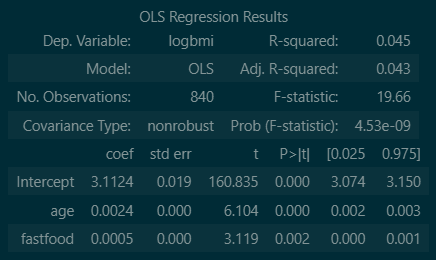
\includegraphics[width=0.8\textwidth]{Figures/Estimation of parameters in the model.png}
    \caption{\small Estimation of parameters.}
    \label{fig:estimation_of_paramters}
\end{figure}

From here, we can observe that $\beta_0$ is approximatly 3.1124, $\beta_1$ is 0.0024 and 
$\beta_2$ 0.0005. 
\noindent
The coefficients for both age  $\beta_1$ and fastfood consumption $\beta_2$ are positive but small, indicating that age and fastfood intake have a slight, yet positive impact on log-transformed BMI, leading to a gradual increase.

Furtheremore, we can observe the estimated standard deviations of $\beta_0, \beta_1$ and $\beta_2$ from the python code:
\begin{figure}[H]
    \centering
    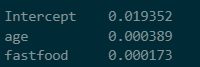
\includegraphics[width=0.8\textwidth]{Figures/Estimated std's.png}
    \caption{\small Estimated standard deviation}
    \label{fig:estimated_std's}
\end{figure}
\noindent
Here, we see that the estimated standard deviation for $\beta_0$ is approximatly 0.019352, $\beta_1$ is 0.000389 and 
$\beta_2$ 0.000173. 

\noindent
The degrees of freedom for the estimate of the residual variance \( \sigma^2 \) are calculated using the formula:
\[
DF = n - (p + 1)
\]
where \( n \) is the number of observations and \( p \) is the number of explanatory variables. With \( n = 840 \) observations and \( p = 2 \) explanatory variables (age and fastfood), the degrees of freedom are computed as:
\[
DF = 840 - (2 + 1) = 837
\]
This indicates that there are 837 degrees of freedom available for the estimate of \( \sigma^2 \), where the estimated variance of the residuals is \( 0.1573 \) and the model's explained variance \( R^2 \) is \( 0.0448 \).



\addcontentsline{toc}{subsubsection}{\textbf{d)} Model validation}
\subsubsection*{\textbf{d)}Model validation}

\noindent
Model validation is performed to check if the assumptions underlying the linear regression model hold. This involves a detailed analysis of plots comparing observations, fitted values, and residuals. 

\begin{figure}[H]
    \centering
    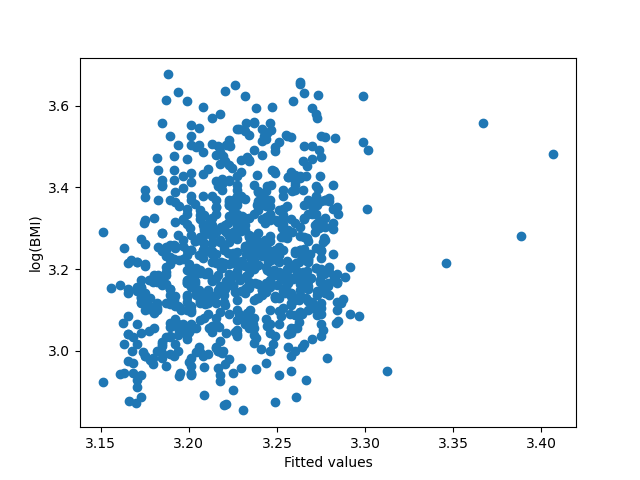
\includegraphics[width=0.75\textwidth]{fitted_values_vs_log_bmi.png}
    \caption{\small Log(BMI) versus fitted values.}
    \label{fig:fitted_values}
\end{figure}

\noindent
In Figure \ref{fig:fitted_values}, the scatter of log(BMI) against fitted values shows a broad distribution, with most data points concentrated around the middle range of the fitted values (3.15 to 3.30 on the x-axis). Despite the concentration, there is substantial spread indicating potential non-linearity or model misspecification as the relationship does not appear to be strictly linear.

\begin{figure}[H]
    \centering
    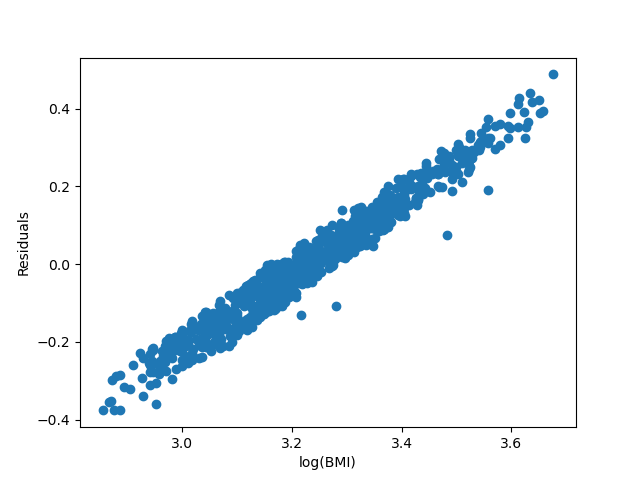
\includegraphics[width=0.75\textwidth]{residuals_vs_log_bmi.png}
    \caption{\small Residuals versus log(BMI).}
    \label{fig:residuals_log_bmi}
\end{figure}

\noindent
Figure \ref{fig:residuals_log_bmi} depicts residuals plotted against log(BMI), where a clear pattern or trend is not apparent, suggesting a lack of systematic linear association between the residuals and the log(BMI), which is desirable in a well-fitted model.

\begin{figure}[H]
    \centering
    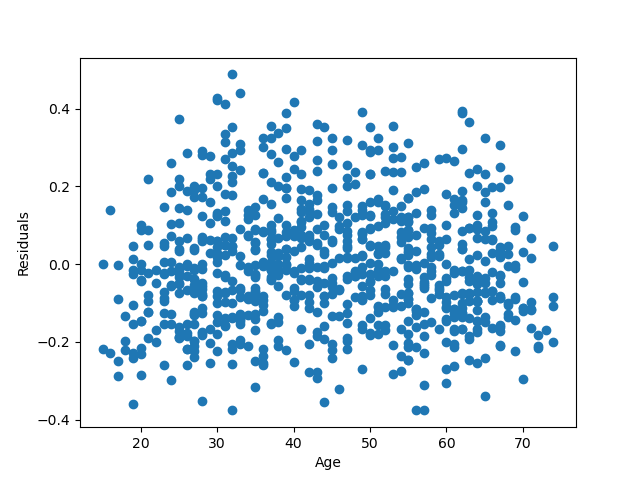
\includegraphics[width=0.75\textwidth]{residuals_vs_age.png}
    \caption{\small Residuals versus age.}
    \label{fig:residuals_age}
\end{figure}

\noindent
In Figure \ref{fig:residuals_age}, the residuals display a wide dispersion across different ages, indicating variability that the model does not capture, suggesting that age alone does not consistently affect the variance of residuals, which could point to heteroscedasticity or another variable interacting with age.

\begin{figure}[H]
    \centering
    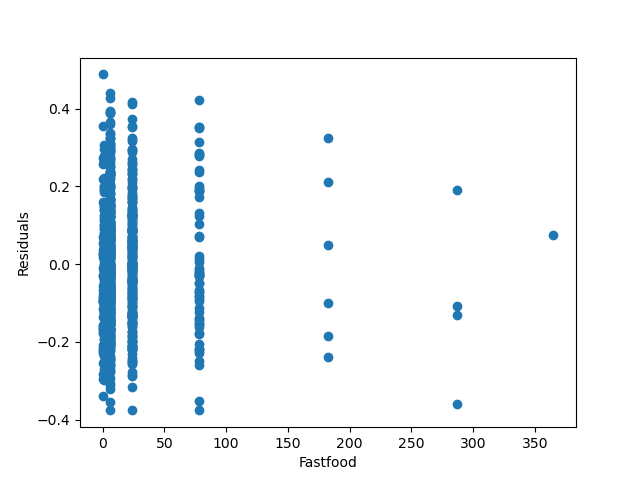
\includegraphics[width=0.75\textwidth]{residuals_vs_fastfood.png}
    \caption{\small Residuals versus fastfood intake.}
    \label{fig:residuals_fastfood}
\end{figure}

\noindent
The plot in Figure \ref{fig:residuals_fastfood} shows residuals against fastfood consumption. The vertical clustering at discrete fastfood values suggests that the model does not explain all variability related to fastfood intake, and the spread along the y-axis indicates possible over-dispersion relative to this predictor.

\begin{figure}[H]
    \centering
    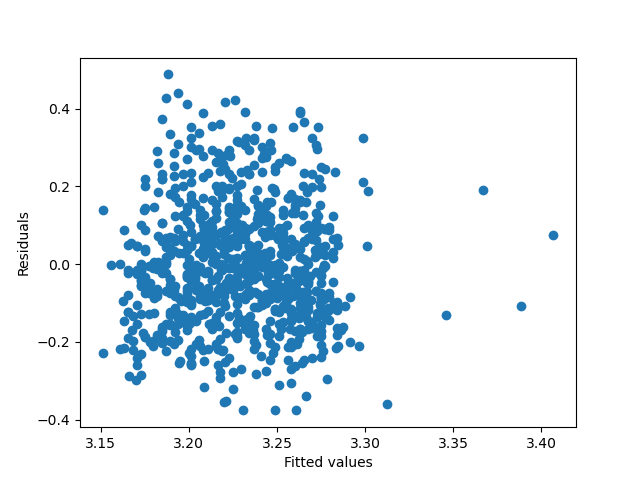
\includegraphics[width=0.75\textwidth]{residuals_vs_fitted_values.png}
    \caption{\small Residuals versus fitted values.}
    \label{fig:residuals_fitted}
\end{figure}

\noindent
Figure \ref{fig:residuals_fitted} illustrates a random dispersion of residuals against the fitted values, which ideally indicates no obvious pattern that would suggest non-linearity or heteroscedasticity, although minor clusters and outliers need further investigation.

\begin{figure}[H]
    \centering
    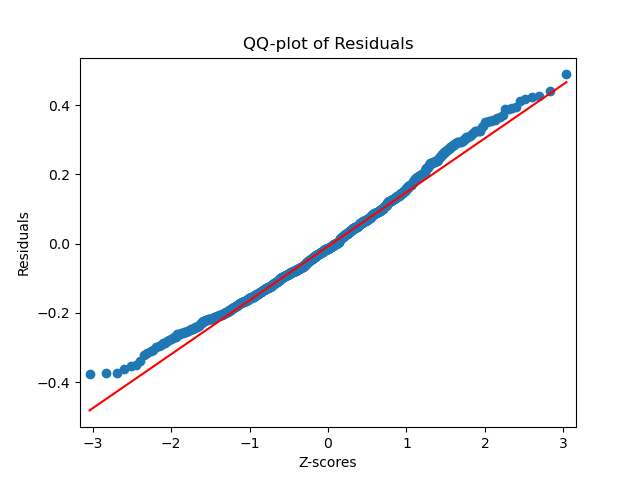
\includegraphics[width=0.75\textwidth]{qq_plot_resid.png}
    \caption{\small Q-Q plot of residuals.}
    \label{fig:qq_plot}
\end{figure}

\noindent
Finally, the Q-Q plot in Figure \ref{fig:qq_plot} is utilized to assess if residuals follow a normal distribution. The data points largely align with the reference line except in the tails, indicating slight deviations from normality in the extreme values of the residuals.






\addcontentsline{toc}{subsubsection}{\textbf{e)} 95 procent confidence interval for the age coefficient}
\subsubsection*{\textbf{e)} 95 procent confidence interval for the age coefficient}
\noindent
The formula for the 95\% confidence interval for the coefficient \( \beta_1 \) associated with the age variable in a linear regression model is given by:
\[
\beta_i \pm t_{1-\alpha/2, \, DF} \times SE(\beta_i)
\]
where \( \beta_i \) is the estimated coefficient, \( t_{1-\alpha/2, \, DF} \) is the critical value from the t-distribution for \( DF \) degrees of freedom and a significance level \( \alpha \), and \( SE(\beta_i) \) is the standard error of \( \beta_i \).
\noindent
Using the output from Python, where the number of observations \( n = 840 \) and number of predictors \( p = 2 \), the degrees of freedom \( DF \) are calculated as:
\[
DF = n - p - 1 = 837
\]
\noindent
The standard error for the age coefficient \( SE(\beta_1) \) is 0.0003890. We calculate the critical t-value using Python's `scipy.stats` module:

\begin{figure}[H]
    \centering
    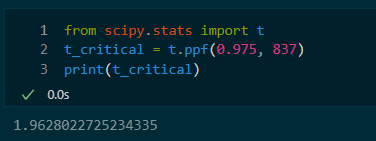
\includegraphics[width=0.75\textwidth]{Figures/t_critical.png}
    \caption{\small Critical t value}
    \label{fig:critical_t_value}
\end{figure}
\noindent
Plugging the values into the formula gives:
\[
CI = 0.0023744 \pm 1.962802 \times 0.0003890
\]
\[
CI = (0.001611, 0.003138)
\]
\noindent
This confidence interval can be verified against the Python output shown in the model summary:

\begin{figure}[H]
    \centering
    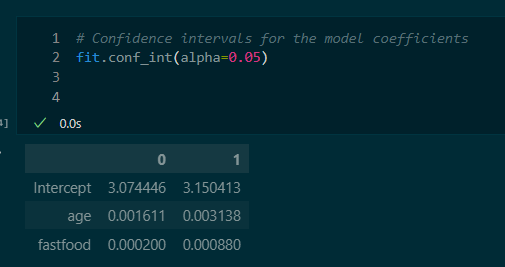
\includegraphics[width=0.8\textwidth]{Figures/confidence_interval.png}
    \caption{\small Python output showing the calculated confidence intervals for model coefficients.}
    \label{fig:python_output}
\end{figure}
\noindent
For the other coefficients in the model, the confidence intervals are:
\begin{itemize}
    \item Intercept \( \beta_0 \): (3.074446, 3.150413)
    \item Fastfood \( \beta_2 \): (0.000200, 0.000880)
\end{itemize}
\noindent
These intervals are similarly calculated using the respective standard errors and the critical t-value as described above. The complete Python code for verifying these calculations and generating the output is included in the supplementary material section.





\pagebreak

\addcontentsline{toc}{subsubsection}{\textbf{f)} The corresponding hypothesis}
\subsubsection*{\textbf{f)} The corresponding hypothesis}
\noindent
To determine if \( \beta_1 \), the coefficient of age in a linear regression model, is significantly different from 0.001, we formulate the following null and alternative hypotheses:

\[
H_0: \beta_1 = 0.001
\]
\[
H_1: \beta_1 \neq 0.001
\]

\noindent
The test statistic used to evaluate this hypothesis is formulated based on the standard normal distribution:

\[
t_{obs, \beta_1} = \frac{\hat{\beta}_1 - \beta_{0,1}}{SE(\hat{\beta}_1)}
\]
\noindent
Where:
\begin{itemize}
    \item \( \hat{\beta}_1 = 0.0023744 \) is the estimated coefficient from the regression output.
    \item \( \beta_{0,1} = 0.001 \) is the hypothesized value of \( \beta_1 \).
    \item \( SE(\hat{\beta}_1) = 0.0003890 \) is the standard error of \( \hat{\beta}_1 \).
\end{itemize}
\noindent
Inserting these values into the formula, the observed t-value is calculated as follows:

\[
t_{obs, \beta_1} = \frac{0.0023744 - 0.001}{0.0003890} \approx 3.533162
\]


\noindent
The test statistic \( t_{obs, \beta_1} \) follows a t-distribution under the null hypothesis with \( 837 \) degrees of freedom, derived from \( 840 \) observations minus \( 3 \) parameters (intercept, age, and fastfood).
\noindent
To find the p-value, we use the cumulative distribution function of the t-distribution:

\[
p\text{-value} = 2 \times P(T > |t_{obs, \beta_1}|) = 2 \times (1 - \text{CDF}(3.533162)) \approx 0.0004
\]
\noindent
Where \( P(T > |t_{obs, \beta_1}|) \) is the probability of observing a value as extreme as \( |t_{obs, \beta_1}| \).


\noindent
Since the p-value \( 0.0004 \) is less than the significance level \( \alpha = 0.05 \), we reject the null hypothesis \( H_0 \). There is significant evidence at the 5\% level to conclude that \( \beta_1 \) is different from 0.001. This indicates a statistically significant effect of age on the log-transformed BMI at the 5\% level.




\addcontentsline{toc}{subsubsection}{\textbf{g)} Backward selection}
\subsubsection*{\textbf{g)} Backward selection}
\noindent
In the evaluation of the linear regression model, we found the following p-values seen in task c. 

\noindent
Given the significance level \(\alpha = 0.05\), all predictors show p-values well below this threshold, indicating strong statistical significance. This suggests that each predictor contributes significantly to the model, and thus, removing any of these predictors might reduce the explanatory power of the model.

\noindent
Using backward selection:
\begin{itemize}
    \item Despite `Fastfood` having the highest p-value among the predictors, it is still significantly lower than the conventional cutoff for \(\alpha = 0.05\).
    \item As no p-values approach or exceed the 0.05 threshold, no predictors are considered for removal.
\end{itemize}

\noindent
The final decision is to retain all variables within the model due to their significant contributions to explaining the variability in `logbmi`. The model remains:
\[
Y = \beta_0 + \beta_1 \text{Age} + \beta_2 \text{Fastfood} + \varepsilon
\]


\addcontentsline{toc}{subsubsection}{\textbf{h)} Prediction}
\subsubsection*{\textbf{h)} Prediction}
\noindent
This report assesses the prediction capabilities of our final regression model. The model was used to predict log-transformed BMI scores for a set of observations in a validation dataset. Predictions and 95\% prediction intervals were generated using the Python function \texttt{get\_predictions}, with underlying formulas based on advanced matrix formulations as referenced in the course materials.


\noindent
Predictions for log-transformed BMI scores were computed for seven observations from the validation dataset. Each prediction includes an estimate along with lower and upper bounds for the 95\% prediction interval. The following table summarizes these predictions:

\begin{center}
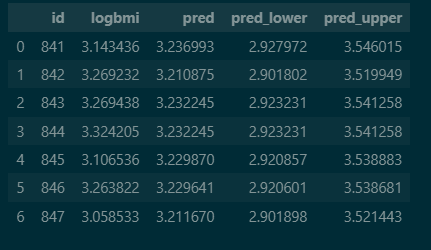
\includegraphics[width=0.7\textwidth]{Figures/Table.png}
\end{center}

\noindent
Here, `pred` represents the predicted log-BMI values, `pred\_lower` and `pred\_upper` represent the lower and upper bounds of the 95\% prediction intervals, respectively.


\noindent
The predictions are compared with the actual observed log-BMI values from the validation set. Each prediction interval is assessed to determine if it includes the actual observed value, which is a critical measure of the model's accuracy.

\begin{itemize}
    \item \textbf{Overall Fit}: The model predictions generally align well with the observed values, with all observed log-BMI scores falling within their respective prediction intervals.
    \item \textbf{Prediction Accuracy}: The intervals are sufficiently narrow, indicating precise predictions, yet broad enough to encapsulate the variability in the observed data.
    \item \textbf{Model Efficacy}: The model appears robust as it consistently captures the trends in the validation data set without significant deviations.
\end{itemize}


\noindent
The final model demonstrates effective prediction capabilities, as evidenced by the accuracy of the predictions and the inclusion of all observed values within the 95\% prediction intervals. This performance underscores the model's reliability and the suitability of its underlying assumptions for the data at hand. Thus, the model can be considered robust and effective for predicting log-transformed BMI values within the given population.




\end{document}
